%% TODO: Add line numbers to motivation example snippets, and update section.

\section{Motivation}
\label{intro:sec}

\subsection{Examples}
\label{examples:sec}

In this section, we present the real-world examples that illustrate
the issues in detecting obsolete TODO comments and motivate our
solution. Figure~\ref{fig:mex_1} displays an example in which the TODO
comment to remind the developers to ensure that the item that is to be
appended to the {\em''Backpack''} menu is a valid game item. This task
was accomplished as the developers added the {\em if-statement} (on
Line \_\_), indicating a concordance between the code-change and the
TODO comment. However, the commit message in this illustration is very
vague, indicating some fix to the {\em''Backpack''} menu, which is not
in accordance with the TODO comment ($T \leftrightarrow C$, $T
\nleftrightarrow M$).

\noindent {\bf Observation 1.} Through this example, we can observe
that the concordance between $T$ and $C$ is important in deciding if
$T$ is obsolete because $T$ and $C$ are at the same level of
abstraction w.r.t. the task. In contrast, $M$ is the subordinate for
$C$, which might not always reliable in precisely describing the code
change $C$. Poor commit messages have been well reported in the
literature~\cite{icse13}. Unfortunately, due to that non-concordance,
the state-of-the-art obsolete TODO comment detection approach,
\tdcleaner \cite{tdcleaner-fse21}, mis-classifies the example of
non-obsolete (i.e., developers have not performed the task).  The
reason is that \tdcleaner is designed to learn the concordance among
all three components $T$, $C$, and $M$.

%Such a non-concordance misleads \tdcleaner towards classifying the
%example as non-obsolete.

%One of the drawbacks in \tdcleaner is that it's designed to learn the
%correlations between inputs of different modalities, i.e., source
%code, and natural language. In this section, we illustrate several
%examples that align with the hypotheses described earlier, where the
%code-change resolves the TODO comment, for which, however, \tdcleaner
%still predicts that it is not obsolete, i.e., has not been performed
%by the developer.

\begin{figure}[t]
	\centering
	\begin{subfigure}{.45\textwidth}
		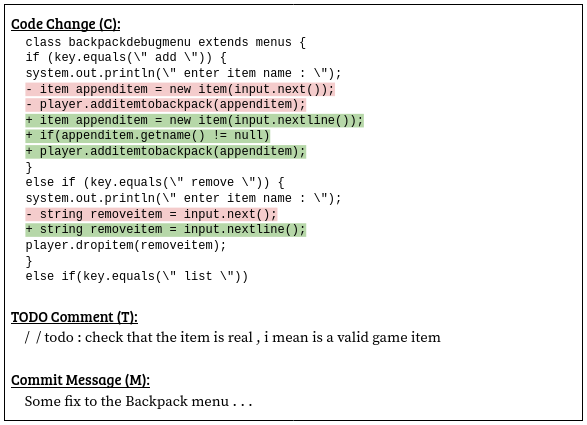
\includegraphics[width=\textwidth]{images/mex_1.png}
		\caption{$T \leftrightarrow C$, $T \nleftrightarrow M$}
		\label{fig:mex_1}
	\end{subfigure}
%%%%%%%%%%%%%%
	\begin{subfigure}{.45\textwidth}
		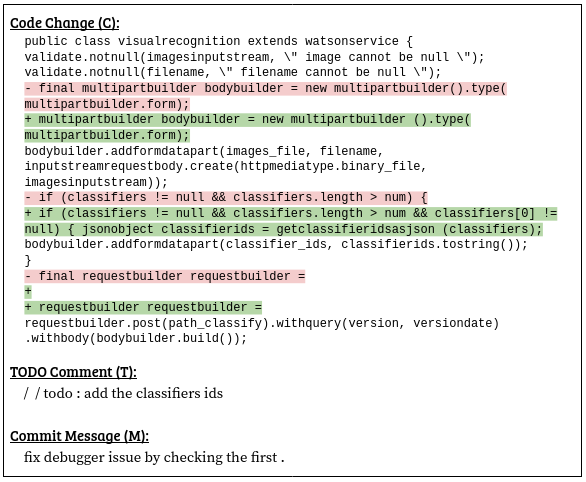
\includegraphics[width=\textwidth]{images/mex_2.png}
		\caption{$T \leftrightarrow C$, $M \geq T$}
		\label{fig:mex_2}
	\end{subfigure}
%%%%%%%%%%%%%%
	\begin{subfigure}{.45\textwidth}
		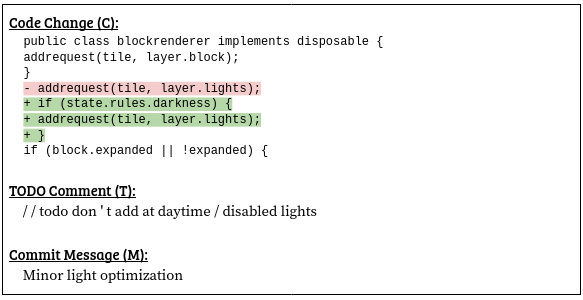
\includegraphics[width=\textwidth]{images/mex_3.png}
		\caption{$T \leftrightarrow C$, $M \geq C$}
		\label{fig:mex_3}
	\end{subfigure}
\caption{Motivating Examples.}
\end{figure}

Figure~\ref{fig:mex_2} illustrates an example in which the TODO
comment is in concordance with the code change, but the commit message
{\em describes other changes in the same commit} as well. The TODO
comment ({\em ``add the classifiers ids''}) reminds the developers to
add classifier IDs, which is clearly addressed in the statement block
within the {\em if-statement} on Line \_\_. However, the code change
in the commit as the whole fixes a debugger issue by adding an
additional condition to the {\em if-statement}, i.e., by also ensuring
that the first element in the classifier is not null. While the commit
message {\em ``fix debugger issue by checking the first.''} aligns
with the code change, the message describes a task overarching the one
in TODO comment.

\noindent {\bf Observation 2.}  In an ``obsolete'' case, the commit
might contain not only the code change for the task in the TODO
comment, but also the change for other tasks, which aligns with the
message logged by the developers: $T \leftrightarrow C$, $M \geq
T$. While the code change $C$ fulfills the task in the TODO comment
$T$, unfortunately, the state-of-the-art \tdcleaner deems this
case as non-obsolete because it considers that the commit message $M$
is not accordance with $T$.

In the example in Figure~\ref{fig:mex_3}, a developer added a TODO
comment, to recommend the team to not add requests to a block at
daytime ({\em ``don't add at daytime / disabled lights''}). This was
addressed by developers' introducing a check for darkness before
adding requests, through the {\em if-statement} on Line \_\_.
However, the commit message logged for this code change was very
general ({\em ``a minor light optimization''}), which does not
precisely capture/summarize the changes in code.

\noindent {\bf Observation 3.} In an ``obsolete'' case, the commit
message $M$ could describe a task that is more general than the code
change $C$ realizing the task described in the TODO comment $T$: ($T
\leftrightarrow C$, $M \geq C$).  Thus, the contextualized vector
learnt for the commit message might have acted as noise, influencing
\tdcleaner to predict that the TODO comment in this case was not
addressed by the developers.

%One of the drawbacks in \tdcleaner is that it's designed to learn the
%correlations between inputs of different modalities, i.e., source
%code, and natural language. In this section, we illustrate several
%examples that align with the hypotheses described earlier, where the
%code-change resolves the TODO comment, for which, however, \tdcleaner
%still predicts that it is not obsolete, i.e., has not been performed
%by the developer.

\subsection{Key Ideas}
\label{ideas:sec}

From the observations, we draw the following ideas to untangle the
triple $<T, C, M>$, and build individual tasks utilizing parts of the
triples, each modeled towards detecting obsolete TODO comments.

%Such inconsistencies motivated us to explore approaches to untangle
%the $<T, C, M>$ triples, and build individual tasks utilizing parts of
%the triples, each modeled towards detecting obsolete TODO
%comments. This idea forms the crux of \tool, which we'll go over in
%more detail in the following sections.

{\bf Key Idea 1 [Text-Code Concordance].} Instead of maximizing $P(S |
\langle T, C, M \rangle)$, we treat $T$ and $C$ as the first-class
information, and $M$ is the subordinate of $C$. $T$ describes the task
that needs to be done. Text-code concordance aims to check if the code
change $C$ realizes the task described in $T$. For example, in
Figure~\ref{fig:mex_3}, the code change with the {\em if-statement} on
Line \_\_ conforms perfectly with the description in $T$ to disabled
lights.
%
Moreover, the code change $C$ might also realize other sub-tasks ($C >
T$). If $C \geq T$, $T$ is considered as obsolete because the code
change already fulfilled the task. For example, in the example in
Figure~\ref{fig:mex_2}, the code changes in the commit fix a debugger
issue by not only adding the classifiers' ids (i.e., the task
described in $T$), but also ensuring the non-null, first element in
the classifier.

{\bf Key Idea 2 [Dual-Task Learning].} Instead of detecting the
concordance among three elements $T$, $C$, and $M$, we decompose it
into two tasks. The first task is {\em text-code concordance} ($T
\leftrightarrow C$ concordance) between $T$ and $C$ as explained. The
second task is {\em sentence-pair concordance} ($T \leftrightarrow M$
concordance) between $T$ and $M$, aiming to classify the concordance
between the task description in $T$ and the description $M$ of the
code change.

With the two key ideas, our approach has the following benefits.
First, the two concordance tasks complement to each other. If $T
\leftrightarrow C$ and $T \nleftrightarrow M$, the text-code
concordance can make the decision on the classification. In contrast,
if $T \nleftrightarrow C$ and $T \leftrightarrow M$, the sentence-pair
concordance can make the decision. Second, we can avoid the incorrect
decisions in the cases illustrated in the motivating examples: ($T
\leftrightarrow C$, $T \nleftrightarrow M$), ($T \leftrightarrow C$,
$M \geq T$), and ($T \leftrightarrow C$, $M \geq C$).

{\bf Key Idea 3 [Ensemble Model with Code Features].} {\color{red}{{\bf Aashish:}
please add the short description on how two tasks are connected via an
ensemble model(?) and how we use code features, instead of text
features in \tdcleaner}}.

 
%key idea 3: model and code features (instead of MLP and text features)
